\section{METODOLOGÍA}\label{sec:methodology}

En este capítulo, se describirá la metodología utilizada para conseguir cumplir los objetivos establecidos. 

Se comenzará por discutir el diseño de la investigación y los métodos de recolección de datos que han sido utilizados para recopilar información. Luego se describirá el enfoque aportado para el preprocesamiento de datos, incluida la limpieza de datos y la selección de características.

Finalmente, se describirán los algoritmos de aprendizaje automático utilizados para el estudio y clasificación de pacientes. 

\subsection{Diseño de Investigación}

Se ha utilizado un enfoque de investigación cuantitativa para examinar la progresión temporal de la bronquiolitis en pacientes pediátricos. Se ha partido de 47 variables descriptivas y de 2 variables que muestran la evolución temporal de los pacientes durante las primeras 24 h de ingreso y que han sido tratadas en el presente trabajo como series temporales. 

\subsubsection{Tipos de Variables}\label{sec:tiposdevariables}

Dentro de las 47 variables descriptivas a utilizar antes mencionadas también se incluyen 4 variables que muestran la evolución temporal por intervalos de los pacientes. Estas variables son:

\begin{itemize}
    \item Flujo de Oxígeno
    \item Frecuencia Respiratoria
    \item Escala SAPI (Sistemas de Alerta Precoz Infantil)
    \item Score Wood-Downes
\end{itemize}

Estas 4 variables no han sido tratadas como series temporales dada la baja frecuencia de recolección durante las primeras 24 h de ingreso; que es el intervalo temporal al que ha sido acotado el estudio. Las tres primeras (Flujo de Oxígeno, Frecuencia Respiratoria y Escala SAPI)variables han sido recopiladas 3 veces durante las primeras 24h del ingreso del paciente pediátrico y la última (Score Wood-Downes) ha sido recogida a la llegada del paciente y a las 24 h. Es decir estas variables describen la estancia del paciente en intervalos.  Estas variables serán catalogadas como \textit{Temporales en Intervalos.} 

Si tratamos estas 3 últimas variables como temporales nos quedarían solamente 36 variables descriptivas. (3 variables temporales $\times$ 3 intervalos + 1 $\times$ 2 intervalos = 11 variables) y por otro lado 2 variables en forma de series temporales. Cada variable de estas contiene 1440 datos. (60 minutos $\times$ 24 horas = 1440).

Dentro de las 36 variables descriptivas restantes se encuentran 3 variables que dan información más allá de las primeras 24 h de monitorización. Estas variables en principio serán excluidas del estudio y son:

\begin{itemize}
    \item Días con Gafas Nasales
    \item Días con O$_2$
    \item Días con OAF
\end{itemize}

Estas 3 variables serán catalogadas como: \textit{Descriptivas fuera del scope}. El \textit{scope} será básicamente las primeras 24 h de ingreso del paciente pediátrico.

Por último dentro de las 33 variables descriptivas dentro del \textit{scope} se encuentran 2 variables que no son ni cualitativas ni cuantitativas. Estas variables serán catalogadas como \textit{Otras}. Las 31 variables restantes serán catalogadas como \textit{Descriptivas dentro de scope}.

En la tabla \ref{tabla:variables_estudio} se muestran las diferentes variables recopiladas para realizar el presente estudio. 

\begin{table}[H]
    \centering
        \begin{tabular}{| m{5cm} | m{1.75cm} | m{7cm} |}
            \hline Tipo de Variable & Cantidad & Nombres  \\ \hline
            Descriptivas dentro de scope & 31 & Edad, Peso, Sexo, Edad Gestacional (EG), Palivizumab, Lactancia Materna (LM), Dermatitis, Alergias, Tabaco, Enfermedad Base, Radiografía, Analítica, Suero, Etiología, Prematuridad, Alimentación, Sonda Nasogástrica, Gafas Nasales al Ingreso, OAF, OAF al ingreso, OAF tras ingreso, Horas de Ingreso tras inicio OAF, UCIP, Deterioro, Pausas de Apnea, PCT (Procalcitonina en la sangre), PCR (Prueba de Proteína C relativa), Leucocitos, Nautrófilos, Linfocitos y Score Cruces Ingreso  \\ \hline
            Descriptivas fuera de scope & 3 & Días con Gafas Nasales, Días con O$_2$ y Días con OAF. \\ \hline
            Temporales en 3 Intervalos & 11 & Frecuencia Respiratoria (0 - 8 h), Frecuencia Respiratoria (8 - 16 h),
            Frecuencia Respiratoria (16 - 24 h),
            Flujo O$_2$ (0 - 8 h),
            Flujo O$_2$ (8 - 16 h),
            Flujo O$_2$ (16 - 24 h),
            SAPI (0 - 8 h),
            SAPI (8 - 16 h), 
            SAPI (16 - 24 h), Score Wood-Downes Ingreso y Score Wood-Downes 24 h . \\ \hline
            Series Temporales & 2 & Frecuencia Cardiaca, Saturación de Oxígeno \\ \hline
            Otras & 2 & Notas e Identificador Paciente. \\ \hline
        \end{tabular}
    \caption{Variables Usadas en el Estudio}\label{tabla:variables_estudio}
\end{table}

Las variables temporales han sido recopiladas durante las primeras 24 h del ingreso del paciente pediátrico cuando mostraba un cuadro bronquiolítico. La frecuencia con la que han sido recopilados los datos ha sido de 1 vez cada minuto. En la siguiente figura \ref{fig:fc-JJB} se muestra un ejemplo de la evolución  variable \textit{Frecuencia Cardiaca} en forma de serie temporal y de la misma forma la figura \ref{satO2-JJB} pero para la \textit{Saturación de O$_2$}. Estas dos series temorales pertenecen a la evolución del paciente pediátrico \textit{JJB\_11182744}.

\begin{figure}[H]
    \centering
    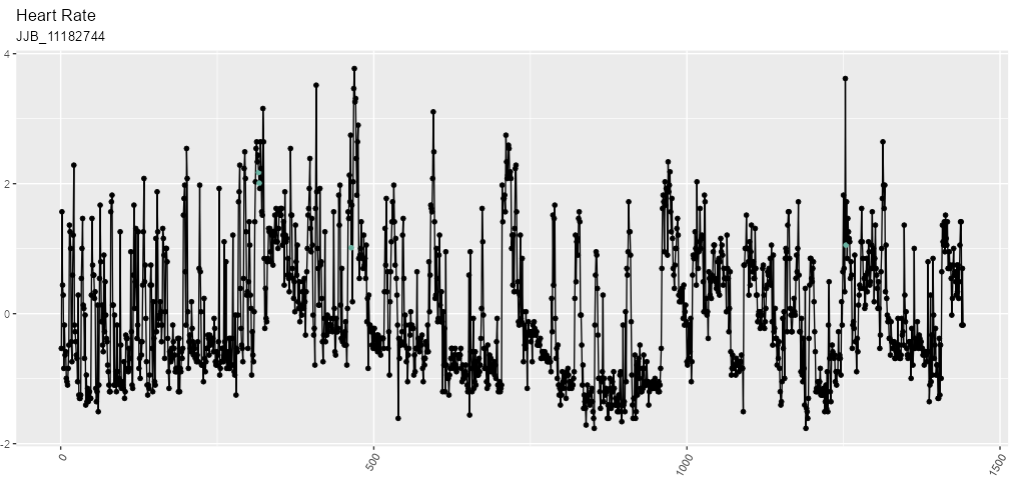
\includegraphics[scale=0.70]{./img/Heart-Rate-JJB.png}
    \caption{Valores de Frecuencia Cardíaca del paciente \textit{JJB\_11182744}}
    \label{fig:fc-JJB}
\end{figure}

\begin{figure}[H]
    \centering
    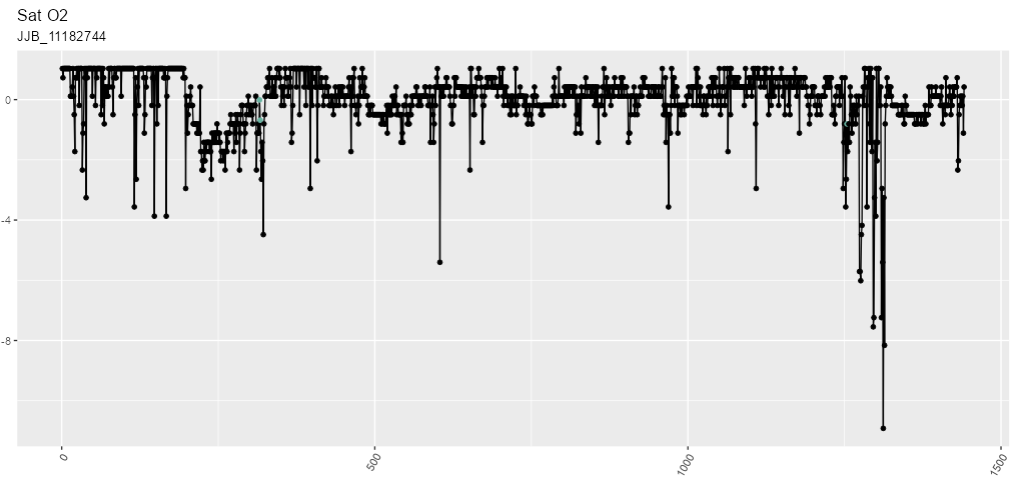
\includegraphics[scale=0.70]{./img/SatO2-JJB.png}
    \caption{Valores de Saturación de O$_2$ del paciente \textit{JJB\_11182744}}
    \label{fig:satO2-JJB}
\end{figure}

A la hora de trabajar con variables temporales se ha de tener en cuenta que los datos temporales pueden ser de dos tipos: \textit{Discretos} o \textit{Continuos}. Los datos discretos son aquellos que se recogen en intervalos de tiempo, por ejemplo, el número de pacientes que llegan a un hospital cada hora. Los datos continuos son aquellos que se recogen de forma continua, por ejemplo, en nuestro caso la saturación y frecuencia cardíaca de un paciente cada minuto.

Para terminar este punto \ref{tiposdevariables} una última cuestión a valorar son las variables cualitativas y cuantitativas que se han recopilado. Las variables cualitativas son aquellas que describen una cualidad del paciente, por ejemplo, el sexo o la edad gestacional. Las variables cuantitativas son aquellas que describen una cantidad del paciente, por ejemplo, la frecuencia cardíaca o la saturación de oxígeno.

En la siguiente tabla se muestra la división entre variables cualitativas y cuantitivas recopiladas en el estudio y dentro del \textit{scope}.

\begin{table}[H]
    \centering
        \begin{tabular}{| m{5cm} | m{1.75cm} | m{7cm} |}
            \hline Tipo de Variable & Cantidad & Nombres  \\ \hline
            Cuantitativas & 15 & Edad, Peso, Edad Gestacional (EG), Horas de Ingreso tras inicio OAF, PCT (Procalcitonina en la sangre), PCR (Prueba de Proteína C relativa), Leucocitos, Nautrófilos, Linfocitos, Frecuencia Respiratoria (0 - 8 h), Frecuencia Respiratoria (8 - 16 h),
            Frecuencia Respiratoria (16 - 24 h),
            Flujo O$_2$ (0 - 8 h),
            Flujo O$_2$ (8 - 16 h),
            Flujo O$_2$ (16 - 24 h). \\ \hline
            Cualitativas & 27 & Sexo, Palivizumab, Lactancia Materna (LM), Dermatitis, Alergias, Tabaco, Enfermedad Base, Radiografía, Analítica, Suero, Etiología, Prematuridad, Alimentación, Sonda Nasogástrica, Gafas Nasales al Ingreso, OAF, OAF al ingreso, OAF tras ingreso, UCIP, Deterioro, Pausas de Apnea, Score Cruces Ingreso, SAPI (0 - 8 h),
            SAPI (8 - 16 h), 
            SAPI (16 - 24 h), Score Wood-Downes Ingreso y Score Wood-Downes 24 h. \\ \hline
            Otras & 2 & Notas e Identificador Paciente. \\ \hline
        \end{tabular}
    \caption{Variables Cualitativas y Cuantitativas Dentro del \textit{Scope}}\label{tabla:cuali_cuanti}
\end{table}

\subsection{Data Collection}

We collected the data for our study from a pediatric hospital, where we recruited infants diagnosed with heart disease. We obtained informed consent from the parents or guardians of the infants before recording the ECG data. The ECG recordings were taken over a period of 24 hours, and we collected a total of X hours of data.

\subsection{Data Preprocessing}

We preprocessed the ECG data using a custom pipeline, which included data cleaning and feature selection. We removed any noisy or missing data from the ECG recordings, and we extracted a set of relevant features that we believed were important for classification of heart rate variability.

\subsection{Machine Learning Algorithms}

We employed several machine learning algorithms to classify the heart rate variability in infants with heart disease. These included Random Forest, Support Vector Machines, and Long Short-Term Memory networks. We trained each model on a subset of the data, and we used cross-validation to assess their performance.

\subsection{Performance Metrics}

We evaluated the performance of each machine learning model using several metrics, including accuracy, precision, recall, and F1 score. We also used confusion matrices and Receiver Operating Characteristic (ROC) curves to assess the models' ability to correctly classify the ECG data.

By following this methodology, we were able to achieve our research objectives and gain insights into the heart rate variability in infants with heart disease. Our results and analysis are presented in Chapter 5.


